\section{Estudio de topologías de arquitecturas}\label{seccion:TopologiaEstudio}
Luego de un estudio exhaustivo del estado de la cuestión (\autoref{chap:estado_del_arte} Página \pageref{chap:estado_del_arte}) se llegó a la conclusión de que las topologias más estudiadas, por ende más maduras y sencillas de aplicar a las activiades que se pretenden realizar en la presente tesis son:
\begin{itemize}
  \item Árbol binario
  \item Red distribuida
  \item Arquitectura hypercube
\end{itemize}

En esta sección, se definirá modelos para medir la confiabilidad de cada una de las topologías de arquitectura que aseguren una mayor tolerancia a fallas a nivel de sistema, de modo tal que si se llega a producir una falla en cualquiera de los nodos (sistemas de procesamiento) de la arquitectura, esta puede reconfigurarse, pemitiendo que esta continúe funcionando, sin sufrir ningún tipo de degradación, aún en la presencia de fallas.

\subsection{Árbol binario}
En primer lugar se planteó un árbol binario de cuatro niveles con backup, basandose en el diseño de \cite{Raghavendra84} \ref{fig:Reliability_binary_tree_4_levels}. Este diseño cuenta con $2^n - 1 =  15$ nodos. De lo estudiado en \autoref{sec:binary_tree} la confiabilidad puede ser calculada de la siguiente manera: $$R_{sys} = R^{2n +1} \prod_{k=0}^{n-1}{[(2^kc+1) - 2^kcR]}$$

Con esto se puede observar la confiabilidad de la red con respecto al tiempo en la Figura \ref{fig:Reliability_binary_tree_4_levels_2}.

\begin{figure}[H]
 \centering
 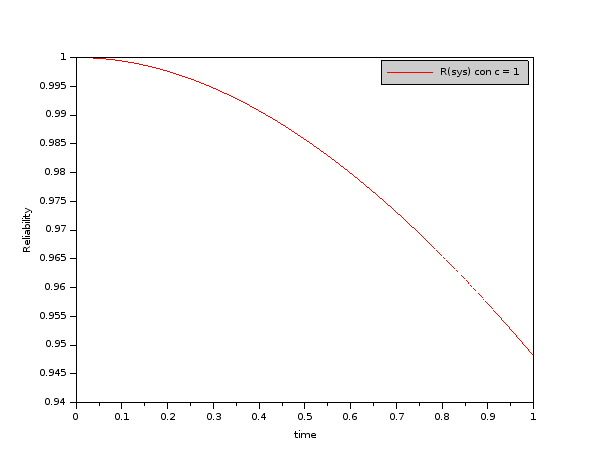
\includegraphics[scale=0.5]{images/Capitulo4/Reliability_BinaryTree.png}
  \caption{Confiabilidad con respecto al tiempo de árbol binario de 4 niveles}
\label{fig:Reliability_binary_tree_4_levels_2}
\end{figure}

La cantidad de niveles que se eligió para esta topología depende del número de subsistemas que se requieren.

Los nodos backup se mantienen inactivos, es decir no participan en el procesamiento durante la vida normal del sistema. En caso de producirse una falla, se supone que estos nodos de redundancia, comienzan a funcionar automáticamente, sin ninún tipo de retraso. Esto, que no corresponde con la realidad, permite simplificar los cálculos para este trabajo de tesis.

\subsection{Red distribuida}
El estudio de una topología de red distribuída no es tan sencilla como la que se plantea para un árbol binario. Para el desarrollo de esta red, además de los 6 nodos que representa cada uno de los subsistemas requeridos, se agrega 2 nodos de redundancia. Por lo tanto se tiene una red de 8 nodos. Siguiendo la metodología de desarrollo presentado por \cite{Pradhan82} se llevó a cabo la red que se presenta en la Figura \ref{fig:distributed_net}.

\begin{figure}[h]
 \centering
 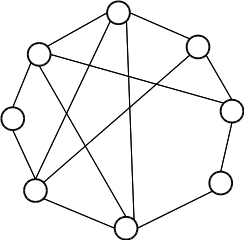
\includegraphics[scale=0.75]{images/Capitulo4/distributed_network.jpg}
  \caption{Red distribuida}
\label{fig:distributed_net}
\end{figure}

Esta cuenta con 4 nodos de grado 4, 2 nodos de grado 3, y 2 nodos de grado 2. Ante cualquier falla de alguno de los nodos de la red, esta topología tiene la capacidad formar subredes, que mantien todos los nodos conectados (a excepción del fallado), asegurandose la funcionalidad y reconfiguración del sistema completo. Estratégicamente y para lograr la condición mencionada anteriormente, se crea la \textbf{condición} de que pueden fallar hasta 4 nodos en simultaneo. Esto aseguraría de que la red continuará funcionando aún en la presencia de fallas (definición de tolerancia a fallas).

Se modificó la fórmula desarrollada  por \cite{Stivaros92}, para lograr coherencia entre los modelos que se plantean en el presente trabajo. Teniendo en cuenta que la confiabilidad del sistema completo es: $$R(t) = \prod_{v \in S} e^{- \lambda t}$$

donde $v$ representa el nodo y $S$ es el subsistema funcional. Es decir, que este modelo recorre todos los nodos funcionales. Cuando existen nodos con fallas, y que dejan de ser funcionales, el modelos es el siguiente: $$R_{sys} =\sum_{i=0}^{k} (( \prod_{v \in S} R(t)) - (\prod_{v \notin S} (1 -  R(t) c )))$$

donde c se definió como una \textit{constante de degradación del sistema} para modelar una degradació del sistema.

En la Figura \ref{fig:reliability_distributedNet} se puede observar la \textit{curva de confiabilidad} del sistema, para el caso en el que todos los nodos se encuentran funcionales.

\begin{figure}[H]
 \centering
 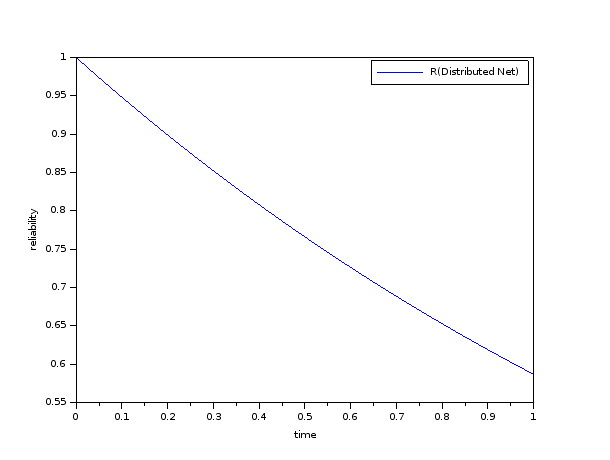
\includegraphics[scale=0.5]{images/Capitulo4/Reliability_DistributedNet.png}
  \caption{Confiabilidad de red distribuida}
\label{fig:reliability_distributedNet}
\end{figure}


Para el caso de la falla de todos los nodos la \textit{curva de confiabilidad} (Figura \ref{fig:reliability_distributedNet_4Nodes_Fail}) muestra correctamente la degradación esperada de la confiabilidad, con respecto al sistema funcionando correctamente sin ninguna falla.

\begin{figure}[H]
 \centering
 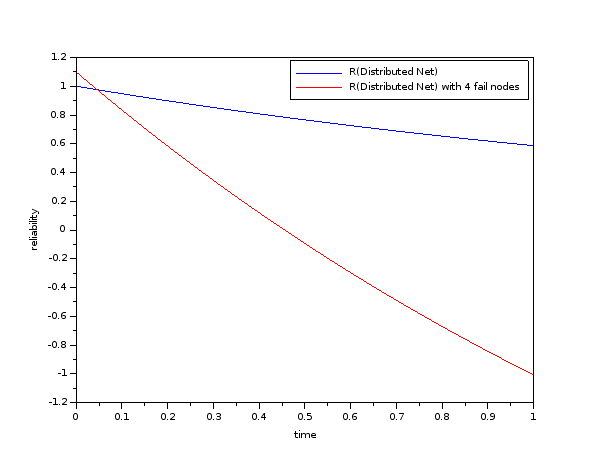
\includegraphics[scale=0.5]{images/Capitulo4/Reliability_DistributedNet_4Nodes_Fail_2.png}
  \caption{Confiabilidad de red distribuida con 4 nodos fallando}
\label{fig:reliability_distributedNet_4Nodes_Fail}
\end{figure}

\subsection{Red hypercube}
Para el caso de la red hypercube se llevaron a cabo modificaciones al modelo planteado por \cite{Mostafa14}, con el propósito de mantener coherencia en los modelos y cálculos que se realizan en este trabajó. Se diseñó una red 3-dimensional, con 8 nodos,  de los cuales 6 nodos corresponden a los diferentes subsistemas y 2 nodos son utilizados de redundancia (Figura \ref{fig:Reliability_Hypercube}).

\begin{figure}[H]
 \centering
 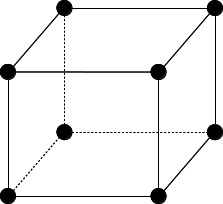
\includegraphics[scale=0.75]{images/Capitulo4/Hypercube2.jpg}
  \caption{Red Hypercube}
\label{fig:Hypercube}
\end{figure}

En este trabajo de tesis, la confiabilidad se calculó por medio del siguiente modelo: $$R_{sys} = 1- [N (1 - e^{- \lambda t}]$$

Como se puede observar el modelo es similar al modelo de árboles binario. Como se pudo estudiar en la bibliografía, árboles binarios y redes hypercube presentan varias similitudes, incluso se emebebe árboles binarios en este tipo de red. La \textit{curva de confiabilidad} de esta red se la puede observar en la fgura

\begin{figure}[H]
 \centering
 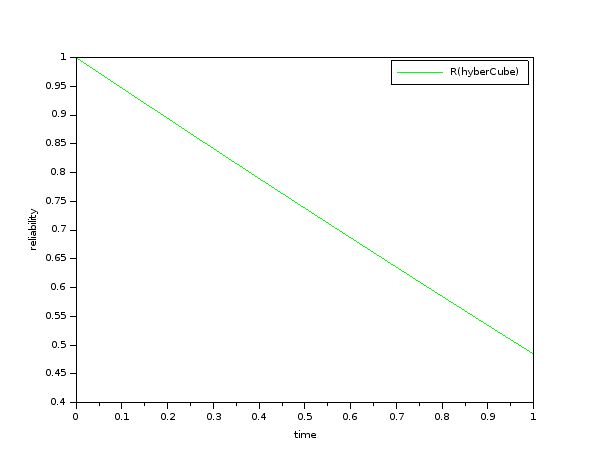
\includegraphics[scale=0.5]{images/Capitulo4/Reliability_Hypercube.png}
  \caption{Confiabilidad de red hypercube}
\label{fig:Reliability_Hypercube}
\end{figure}

\section{Topología utilizada en la arquitectura a diseñar}

Teniendo en cuenta los modelos presentados anteriormente, se procede a realizar una comparación de las diferentes curvas. El resultado de esto, permitiré conocer de manera analítica qué topología presenta una mayor tolerancia a fallas a travez del tiempo. Además, teniendo en cuenta lo estudiado en el estado de la cuestión, se puede realizar una comparación conceptual de las tres topologías.

La aplicación de árboles binario podríar resultar una buena opción, ya que representa un desarrollo sencillo. En contraposición se puede indicar que existe un alto grado riesgo de que se produzca una falla en el nodo raíz y de su redundancia, lo cual pondría en peligro la misión. Así mismo, presenta otro punto negativo que se puede mencionar y es la gran cantidad de enlaces que esta necesita para mantener a todos los nodos de la red conectados.

Por otra parte, la red distribuída cuenta con la capacidad de distribuir el trabajo en todos sus nodos. Esto quiere decir, que si se produce una falla irrecuperable en cualquiera de sus nodos, la arquitectura podría continuar funcionando sin verse afectada por la ausencia de dicho nodo. Esto demanda un procesamiento computacional extra, y la necesidad de desarrollar algorimtos de ruteo especiales. Además, como punto negativo se puede mencionar que también, al igual que los árboles binarios, necesitan una gran cantidad de enlaces.

Por último, las topologías hypercube tiene un excelente respaldo teórico, exigen menor cantidad de enlaces, y pueden tolerar la falla de una gran cantidad de nodos (hasta el 50\% de los nodos). Su complejidad aumenta en gran medida, cuando se desarrollan arquitecturas de más dimensiones, sin embargo, esto aumenta su confiabilidad.

Como se mencionó en el primer párrafo, se realizó una comparación de módelos de confiabilidad de las tres topologías estudiadas. Se asumió que la distribución de la confiabilidad es exponencial, con una tasa de falla fija de 1/15, y se estudió su evolución en un rango $[0,1]t$. El resultado de esta comparación se la puede observar en la Figura \ref{fig:comparative_reliablities} y en la Tabla \ref{table_comprative_reliability}.

Se observa que tanto las redes distribuidas como la hypercube presenta una mayor confiabilidad a través del tiempo que  los árboles binarios. Si bien, las redes distribuidas y la hypercube tienen una curva similar, la primera presenta una mayor confiabilidad sostenida en el tiempo.

\begin{figure}[H]
 \centering
 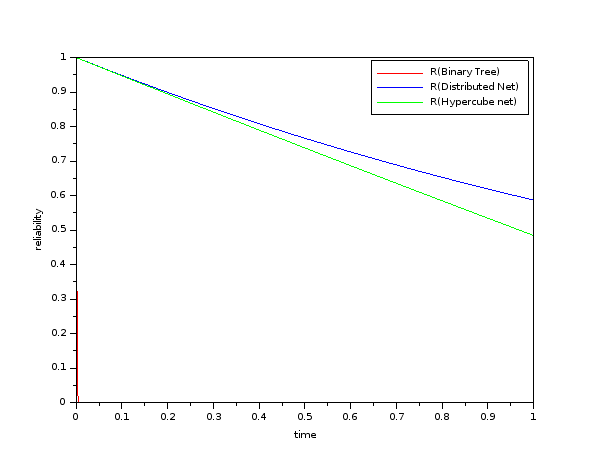
\includegraphics[scale=0.5]{images/Capitulo4/comparative_reliablities.png}
  \caption{Comparación de confiabilidad}
\label{fig:comparative_reliablities}
\end{figure}

\begin{table}[H]
\centering
\caption{Comparación de confiabilidad de topologías}
\label{table_comprative_reliability}
\begin{tabular}{r|r|r|r|}
\cline{2-4}
\multicolumn{1}{l|}{} & \multicolumn{3}{c|}{Topologías de red} \\ \hline
\multicolumn{1}{|c|}{T} & \multicolumn{1}{c|}{Tree Net} & \multicolumn{1}{c|}{Distr Net} & \multicolumn{1}{c|}{Hyper Net} \\ \hline
\multicolumn{1}{|r|}{0} & 1 & 1 & 1 \\ \hline
\multicolumn{1}{|r|}{0.001} & 0.803766 & 0.999947 & 0.999947 \\ \hline
\multicolumn{1}{|r|}{0.002} & 0.64604 & 0.999893 & 0.999893 \\ \hline
\multicolumn{1}{|r|}{0.003} & 0.519265 & 0.99984 & 0.99984 \\ \hline
\multicolumn{1}{|r|}{0.004} & 0.417368 & 0.999787 & 0.999787 \\ \hline
\multicolumn{1}{|r|}{0.005} & 0.335466 & 0.999733 & 0.999733 \\ \hline
\multicolumn{1}{|r|}{...} & ... & ... & ... \\ \hline
\multicolumn{1}{|r|}{0.995} & 0 & 0.948317 & 0.947109 \\ \hline
\multicolumn{1}{|r|}{0.996} & 0 & 0.948266 & 0.947056 \\ \hline
\multicolumn{1}{|r|}{0.997} & 0 & 0.948216 & 0.947003 \\ \hline
\multicolumn{1}{|r|}{0.998} & 0 & 0.948165 & 0.94695 \\ \hline
\multicolumn{1}{|r|}{0.999} & 0 & 0.948115 & 0.946897 \\ \hline
\end{tabular}
\end{table}


Con esto se puede concluir que la topología que presenta un mayor grado de confiabilidad es la que responde a una filosofía distribuida (bajo las condiciones en las que fueron estudiadas). Por lo tanto, la arquitectura satelital, tolerante a fallas y basada en componentes COTS que se desarrolla en la presenta tesis se basa en una \textbf{topología distribuída} para interconectar los diferentes subsistemas.

\section{Topología propuesta}
Sobre la base de los resultados presentados en \citep{Arias17} se puede establecer que la topoloǵia propuesta es la más adecuada para el desarrollo de una arquitectura tolerante a fallas como se presenta en la Figura \ref{fig:topo_propuesta}. En esta se puede observar que cada subsitema (térmico, power, telemetría, etc.) tiene su propia CPU controladora. Estas CPU se conectan a los nodos.

\begin{figure}[h!]
 \centering
 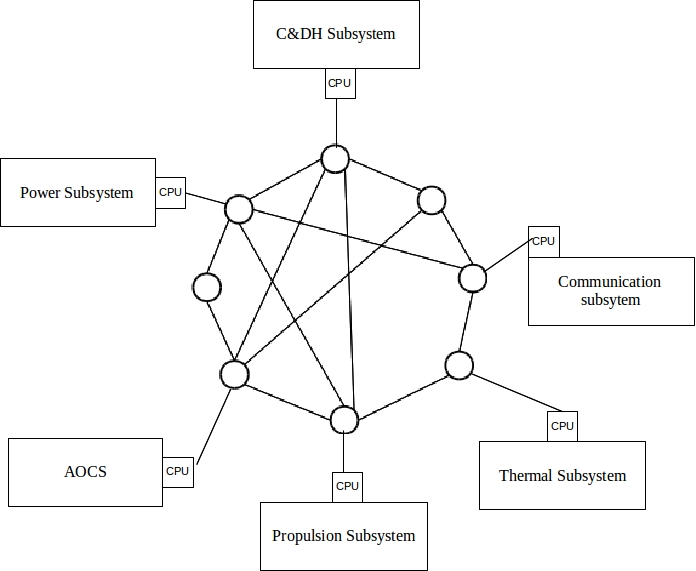
\includegraphics[scale=0.5]{images/Capitulo4/arq_final.jpg}
  \caption{Arquitectura propuesta utilizando topología de red distribuida}
\label{fig:topo_propuesta}
\end{figure}

El modelo exige como requerimiento que cada nodo debe estar compuesto por una computadora (componente COTS) que es la encargada de realizar el procesamiento de las tareas. También, debe exitir un puente de comunicación entre la red y la CPU del subsistema. De este modo se hace frente a posibles fallas en la computadora del nodo. Esta conexión se observa en la Figura \ref{fig:conn_prop}

\begin{figure}[h!]
 \centering
 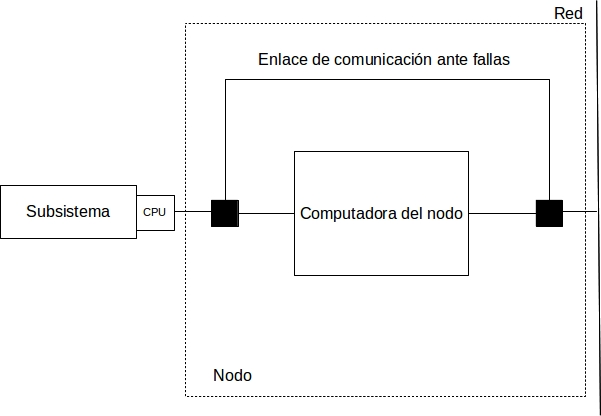
\includegraphics[scale=0.3]{images/Capitulo4/com_nodo.jpg}
 \caption{Conexión entre la red y el subsistema}
\label{fig:conn_prop}
\end{figure}
